\section{Metadatenmodell}

Wie bereits erwähnt muss ein Modell erstellt werden, dass die Metadaten abbildet, die bei einer Ingestion erfasst werden (\cref{fig:datenmodell}).
Zu diesen Metadaten gehören alle Informationen über die Herkunft der Daten, also die Datenquelle und das Speicherziel.
Diese werden zum Großteil in für Spark erforderlichen Parametern widergespiegelt.
Ein weiterer Teil der Metadaten sind alle Informationen über die Ausführung einer Ingestion.

\subsection{DatasourceDefinition}

Das Metadatenmodell beschreibt eine Datenquelle und hat als zentrales Element das Konzept DatasourceDefinition.
Ein Teil des Modells besteht aus Feldern, die für Spark erforderlichen Informationen enthalten.
Dazu gehören: \begin{itemize}
    \item zusätzliche Abhängigkeiten für Spark (spark.jars.packages),
    \item das Format und Optionen für die Reader und
    \item bei benutzerdefinierten Speichersystemen das Format, die Optionen und einen Schreibmodus für die Writer.
\end{itemize}
Neben den Spark spezifischen werden noch folgende weitere Informationen erfasst: \begin{itemize}
    \item ein Name für die Datenquelle,
    \item wenn eine Update-Quelle erstellt wird, die Id der Datenquelle, welche die Update-Quelle aktualisieren soll,
    \item das Datum der Erstellung und letzten Änderung,
    \item den Namen der Id-Spalte in den Daten (wird später für die Deltaberechnung benötigt),
    \item den Typ, der zu lesenden Daten,
    \item eine Liste der zu laden Dateien, wenn es sich um eine Datei-Ingestion handelt,
    \item den Typ, wie die Daten geschrieben werden,
    \item eine Liste mit der Zeitsteuerung für eine kontinuierliche Ingestion,
    \item eine Liste mit Plugindateien und
    \item eine Liste mit Abhängigkeiten der Plugins.
\end{itemize}

Die möglichen Lese-Typen ergeben sich aus der Betrachtung, wie die Daten in das Data-Lake-System gelangen und welche Struktur sie haben.
Bei einer Pull-Ingestion ist das System dafür verantwortlich Daten aus einer Quelle zu laden.
Dies ist zum Beispiel bei Datenbanken der Fall.
Das Gegenteil dazu ist eine Push-Ingestion, bei der die Daten direkt an den Data Lake gesendet werden.
Diese muss jedoch nochmal in zwei unterschiedliche Typen unterteilt werden.
Bei einer Stream-Ingestion, also bei Datenströmen, werden kontinuierlich neue Daten an das System gesendet.
Und bei einer File-Ingestion werden Dateien hochgeladen, welche die Daten enthalten, wobei wichtig ist, dass alle Dateien das gleiche Dateiformat und je nach Typ eine ähnliche oder gleiche Struktur haben.
Die Dateien können sich in Daten- und Quelldateien unterscheiden.
Datendateien enthalten unstrukturierte Daten und werden einfach im HDFS mit abgelegt, ohne weiter verarbeitet zu werden.
Das könnten zum Beispiel Bilder oder Videos sein.
Quelldateien enthalten mindestens semistrukturierte Daten und dienen dem Zweck, in ein anderes Speicherformat, wie zum Beispiel Parquet oder eine Delta-Tabelle geschrieben zu werden.
Es ist nicht möglich, Daten direkt an die API zu senden.
Alle Push-Ingestions sollen über diese beiden Typen abgebildet werden.

Die möglichen Schreib-Typen werden aus den Speicherzielen abgeleitet.
Custom bedeutet, dass der in der DatasourceDefinition konfigurierte Speicher verwendet werden soll.
Delta ist das Speichern im internen Speicher aber mit einer Versionierung und Default ist das Speichern ohne Versionierung.

Für die Umsetzung einer unkomplizierten Versionierung der DatasourceDefinition werden alle veränderlichen Informationen in Revisionen gespeichert.
Das betrifft alle oben genannten Felder.
Die Revisionen einer DatasourceDefinition erhalten eine fortlaufende Nummer.
Die DatasourceDefinition selbst hält dann nur noch eine Liste aller Revisionen und die Nummer der aktuellen.

\subsection{IngestionEvent}

Das Modell für den Ablauf einer Ingestion ist das IngestionEvent.
Dieses enthält, wie die Revision, eine fortlaufende Nummer, ein Start- und Enddatum, den aktuellen Status indem es sich befindet, die Nummer der Revision mit der es gestartet wurde und eine Fehlernachricht, falls ein Fehler aufgetreten ist.

Das IngestionEvent kann auch zur DatasourceDefinition hinzugefügt werden.
Dafür werden Felder hinzugefügt, die alle IngestionEvents, die Nummer des letzten und die Nummer des letzten erfolgreichen IngestionEvents enthalten.

\begin{figure}
    \centering
    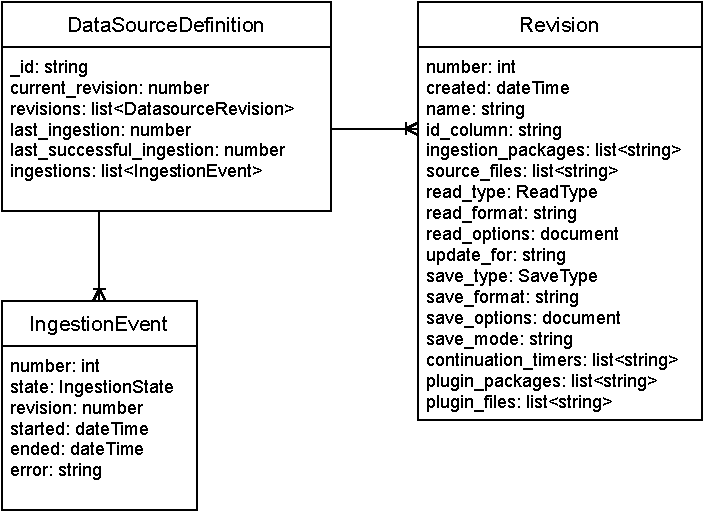
\includegraphics{Grafiken/Entwicklung-Datenmodell.pdf}
    \caption{Übersicht Metadatenmodell}
    \label{fig:datenmodell}
\end{figure}